%Yiru
%Take information from project abstract
\section{Introduction to Use Case and Datasets}
\subsection{Use Case}
In this project, our purpose is to integrate a dataset about companies with another dataset about cities their headquarters are located in. However, in order to gather more information about companies, first we combine several datasets together, which are all about companies but come from different sources. Then we will integrate this result with location. As such the resulting integrated dataset may be used for additional information regarding companies and their location around the world.

%not sure if we need this part
%First, we gather data from each data source. For most datasets we write queries for different web services(DBpedia and Freebase) to request data about companies and location. One dataset is provided as .xls file, so we transfer it into .csv file for mapping. Since a company might have abbreviation in each dataset, we do some transformation on name and country.\\
%In second phase, we identify a company in multiple datasets by their overlapping attributes. In order to reduce the comparing time, we use country as blocking key in most situations.\\
%Then, by using specific resolution strategies for each attribute, we solve the conflicting information about companies. In the end these datasets can be merged together and represented in the form of our integrated target schema.\\
%

\subsection{Datasets}
In order to collect suitable data we tried different data service providers such as Datahub, finally we have collected total four datasets from three different sources and in three different formats, including: 
\subsubsection{Forbes:Company}
Forbes is an American business magazine and it is well known for its lists and rankings, including its lists of the richest Americans (the Forbes 400) and rankings of world's top companies (the Forbes Global 2000). The ranking is based on a mix of four metrics: sales, profit, assets and market value. This dataset contains 2000 companies during the period 2000 to 2014 and 7 attributes which describes these companies information.
\subsubsection{DBpedia:Company}
The information of company is extracted from DBpedia, since it provides relatively complete information.  To access information from DBPedia we used the public SPARQL endpoint (at http://dbpedia.org/sparql). Figure 1.1 is our query for company, actually there is total 764398 companies in DBpedia, which would be too much for us and also not easy to handle it in terms of processing time and space. In order to reduce the number of data, we limit the company types to "company" and "public company" and only extract the companies that provide attributes "LocationCity" and "LocationCountry", these two attributes can also be related with Location Information, that's why we consider them as necessary and others are optional. On the other hand, if all these attributes are necessary, there will be only few thousands companies extracted, because not all companies have all these nine attributes, in this case few overlapping data will be in the final integration results. In addition to this, as many attributes such as KeyPeople, locationCity have multiple values which result in the same company would appear more than one times, to avoid these duplicates we used "group\_contac", a function in Sparql, to group many value together. There are also many values for Revenue but without date notation, so we just took the maximum value. 

\begin{figure}[H]
	\begin{center}
	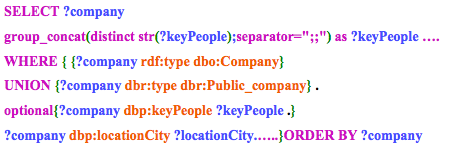
\includegraphics[width=10cm]{DB_Com}
	\caption[DBpedia Query For Company]{DBpedia Query For Company}
	\label{fig:db}
	\end{center}
\end{figure}

\subsubsection{Freebase:Company}
Freebase provides a web service to query data and return in JSON. The total number of entities is 3,182. We make name nonoptional, since we want to use it to compare companies in each dataset. Also, \texttt{number\_of\_employees} is nonoptional, because the amount for being optional is around 230,000 and we don't want to use it. The rest attributes are all optional.
First we test queries on the query page to make sure we get the right data. Then, we build a Java project to execute the MQL Read API. Additionally, during the mapping procedure, we occur some problem about multiple values in JSON array and JSON object, it couldn't match in target schema because of the various number of values. Thus, we convert them into one string and separate with two semicolons while excuting Java project.

\subsubsection{DBpedia:Location}
%Silvia/Zehui
We also extracted Location information from DBpedia with the same method as Company. Figure 1.2 is the query for location. For the same reason as Company, we limit the location types to "city" and "AdministrativeRegion", which are more relevant to our company dataset. Also some attributes have many values without extra information, it's hard to identify which one represents the current state, thus, we just took the maximum number of them among multiple values. Furthermore, the name of locations are provide in different languages, while in our project we just focus on english, so we filtered language as english.